\documentclass[11pt]{amsart}
\usepackage{geometry}                % See geometry.pdf to learn the layout options. There are lots.
\geometry{letterpaper}                   % ... or a4paper or a5paper or ... 
%\geometry{landscape}                % Activate for for rotated page geometry
%\usepackage[parfill]{parskip}    % Activate to begin paragraphs with an empty line rather than an indent
\usepackage{graphicx}
\usepackage{amssymb}
\usepackage{epstopdf}
\usepackage [autostyle, english = american]{csquotes}
\usepackage{hyperref}
\MakeOuterQuote{"}
\DeclareGraphicsRule{.tif}{png}{.png}{`convert #1 `dirname #1`/`basename #1 .tif`.png}

\title{Project 6: Simple Solution to an Second Order Differential Equation Using a Mean Value Theorem Approximation}
%\author{Jessica Bartley}
%\date{}                                           % Activate to display a given date or no date

\begin{document}
\maketitle
%\section{}
%\subsection{}

This project is about solving a second order differential equation using the mean value theorem (or as it was called in class, a "symmetric three point approximation method").  We will do this by taking this second order differential equation and writing it as two coupled first order differential equations.  The second order differential equation (which happens to describe the motion of a driven pendulum) is:

\begin{equation}
\frac{d^{2} \theta}{d t^{2}} + \sin{\theta} = a \cos{\omega t}
\end{equation}
\vspace{2 mm}

Where $t$ is time, $\theta$ is the angle the pendulum makes with the vertical, and $\omega$ is a frequency of the driving force.  The right hand side of this expression describes the driving force.  We can make the substitutions $y_1 = \theta$ and $y_2 = \frac{d y_1}{d t}$ so as to arrive at the two coupled first order differential equations:

\begin{equation}
\frac{d y_1}{dt} = y_2
\end{equation}
\begin{equation}
\frac{d y_2}{dt} = a \cos{\omega t}- \sin{y_1}
\end{equation}
\vspace{2 mm}

\textbf{The goal of this code is to plot three graphs: $y_1$ vs $t$ (angle vs time), $y_2$ vs $t$ (angular velocity vs time), and $y_1$ vs $y_2$ (angle vs angular velocity).}
\newline

We will use the mean value theorem when considering the derivatives of $y_1$ and $y_2$.  Although this code does not actually estimate $\frac{d y_1}{dt}$ or $\frac{d y_2}{dt}$ at any specific value, we use the derivative approximation formula (Eq 4) to solve for specific instances of $y_1$ and $y_2$.  These values will give a recursion relation that allows us to plot the required graphs.
\newline

\begin{equation}
f \prime (x_0) = \frac{f(x_0 + h) - f(x_0 - h)}{2h}
\end{equation}
\vspace{2 mm}

Where $x_0$ is the middle point of interest and $h$ is the distance between points.
\newline

In general, we can estimate the derivative of any function $f$ at the value $x_0$ if we know one point on the function to either side of $f(x_0)$.  The derivative $f \prime (x_0)$ is estimated by the slope of the secant line connecting the two symmetric points.  If the function is continuous and differentiable on the interval then the mean value theorem, illustrated in Fig 1, guarantees that there exists a point somewhere between $x_0 - h$ and $x_0 +h$ that has a tangent line equal to the slope of the derivative.  We are approximating the slope at  $x_0$ as this secant slope.
\newline

\begin{figure}[ht!]
\centering
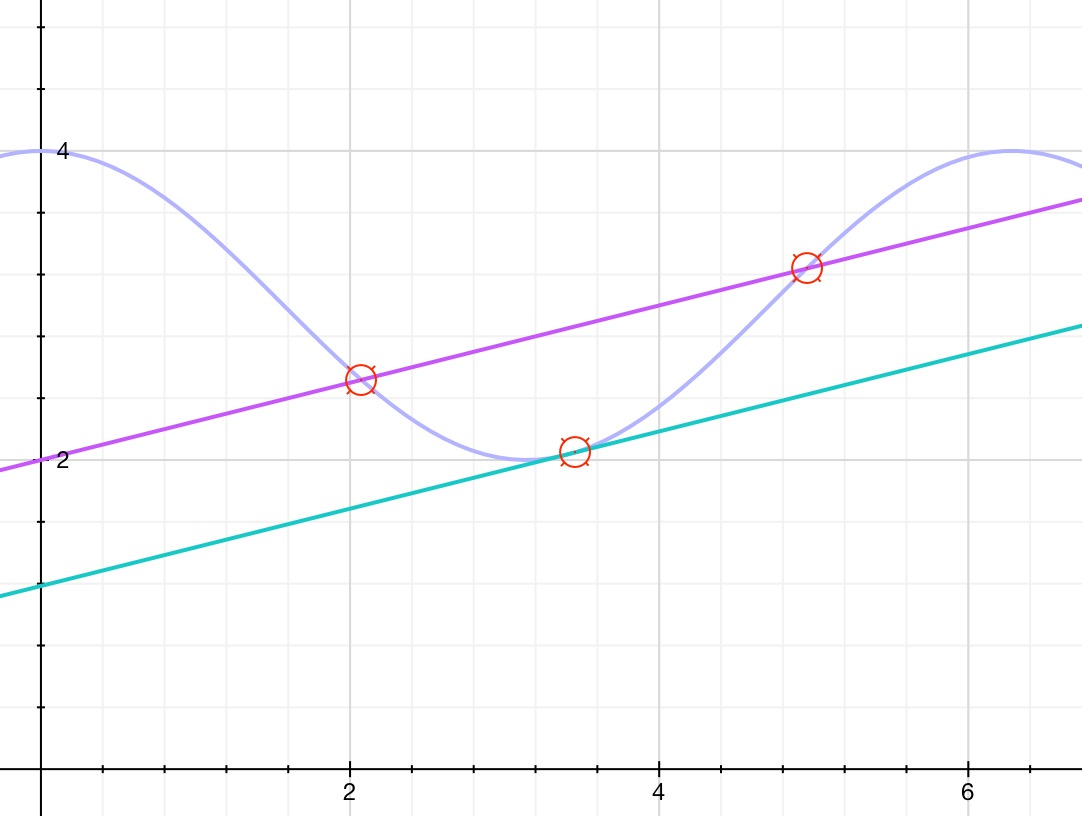
\includegraphics[width=120mm]{MeanValueTheorem.jpg}
\caption{We use the mean value theorem to approximate the derivative of some function evaluated at the midpoint between two bounds.}
\label{overflow}
\end{figure}

\vspace{3 mm}

Now, it is important to note that for this code we are never actually approximating a derivative.  When we apply Equation 4 to $y_1$ and $y_2$ (defined in Equation 2 and 3) and rearrange we get:

\begin{equation}
y_1(t+h) = 2h y_2(t) + y_1(t-h)
\end{equation}

\begin{equation}
y_2(t+h) = 2h \left[- \sin{y_1(t)}+a \cos{\omega t} \right] + y_2(t-h)
\end{equation}
\vspace{2 mm}

This is our recursion relation.  We will start with some initial conditions and use these equations to step $y_1$ and $y_2$ forward so that we find these functions at sequential values of t.  Then we will plot $y_1$ vs $t$, $y_2$ vs $t$, and $y_1$ vs $y_2$.  The latter of which should be an ellipse.
\newline

Note, this is not an ideal method to numerically solve differential equations.  Because of this we will see discretization error propagate across our results.  If this error did not exist then our $y_1$ vs $y_2$ graph would be a periodic ellipse.  It actuality this graph will not be periodic, but it should look something like an ellipse at the beginning.
\newline

The steps for the code include:
\begin{enumerate}
\item  Declaring the initial conditions $y_1(0)=0$, $y_2(0)=0$, $y_1(-h)=0$, ,$y_2(-h)=0$ and another other parameters such as $\omega$ or $h$.
\item Calculating $y_1(t+h)$ and $y_2(t+h)$ via Equations 5 and 6.  We will loop through this step to get out many sequential values of $y_1$ and $y_2$.
\item Then we plot the graphs.
\end{enumerate}


\end{document}  